\documentclass[hidelinks]{article}
%
%%%%%%%%%%%%%%%%%%%%%%%%%%%%%%%%%%%%%%%%%%%%%%%%%%%%%%%%%%%%%%%
% START CUSTOM INCLUDES & DEFINITIONS
%%%%%%%%%%%%%%%%%%%%%%%%%%%%%%%%%%%%%%%%%%%%%%%%%%%%%%%%%%%%%%%
%
\usepackage{amsmath}
\usepackage{parskip} %noident everywhere
\usepackage{hyperref} % Show hyperlinks - claudio
\hypersetup{
    colorlinks = true
    linkcolor = blue
    urlcolor = red
    }
% Block diagrams
\usepackage{tikz}
\usetikzlibrary{shapes.geometric, arrows, calc}
\tikzstyle{block} = [rectangle, draw,
    text centered, rounded corners, minimum height=3em, minimum width=6em]
\tikzstyle{sum} = [draw, circle, node distance=1cm]
\tikzstyle{input} = [coordinate]
\tikzstyle{output} = [coordinate]
\tikzstyle{arrow} = [draw, -latex']
\usepackage[left=0.75in, right=0.75in, top=0.5in, bottom=1in]{geometry}
\usepackage{graphicx}
\usepackage{subcaption}
\usepackage{titlesec}
%
%%%%%%%%%%%%%%%%%%%%%%%%%%%%%%%%%%%%%%%%%%%%%%%%%%%%%%%%%%%%%%%
% END CUSTOM INCLUDES & DEFINITIONS
%%%%%%%%%%%%%%%%%%%%%%%%%%%%%%%%%%%%%%%%%%%%%%%%%%%%%%%%%%%%%%%
%
\pdfobjcompresslevel=0
%
\title{\vspace{-1cm} Finite Elements Report}
\author{\vspace{-2cm} Claudio Vestini}
\date{}
\begin{document}
\maketitle
%
\paragraph{Introduction}
This practical was concerned with applying Boundary Conditions (BCs) to \texttt{problem inc 1.m} for solving a plane stress equilibrium problem of a stretched bar.
The study follows a structured approach: we first identified the formulation of the BCs in the codebase, modified it to specify Dirichlet BCs for the left and right edges of the bar, then verified the undeformed state. A final combined loading case was finally tested.
Horizontal stress $\sigma_x$ and plane strains are visualised, using a $10^7$ scaling factor to make small deflections visible.
Values of $\sigma_x$, as well as those of all loads, deflections and scaling factors, have been chosen arbitrarily.

\paragraph{Identification of BCs and Undeformed State}
BCs are defined in the original codebase at lines 23-33 of \texttt{problem inc 1.m}. The code concatenates the left edges' degrees of freedom (DoFs) into the \texttt{prescribedDoF} array, which is initially fixed to provide zero displacements. This constitutes a Dirichlet boundary condition for the left edge, (note: no condition is initially imposed on the right edge). Force vectors $Fs$ and $Fb$ (which represent, respectively, applied and body forces) are both initialised to zero. This ensures the top and bottom edges are traction-free.

The undeformed state is then obtained by running the code, and is not included here due to lack of space.
\paragraph{Modifying BCs}
We were asked to implement a Dirichlet BC for the right edge of the bar, with an arbitrary fixed displacement. We obtained this by first including the relevant nodes for the right edge in the \texttt{prescribedDoF} array. We then specified a fixed horizontal displacement to the right edge by assigning an arbitrary value to \texttt{u prescribed(rightXDoF)} (the value itself is not relevant to the discussion), whilst also ensuring the vertical YDoF was set to zero. The result was the stretched bar of Figure~\ref{fig:stretch}.

The second load case required combined stretch + bending (the details of how to obtained this were omitted from the problem statement). I implemented this load case by setting the balue of $Fs$ to a constant positive value (applying a distributed force acting upwards). The Dirichlet BCs were left unchanged from the previous part. The results are shown in Figure~\ref{fig:bending}.
%
\begin{figure}[h]
    \centering
    \begin{subfigure}[t]{0.49\textwidth}
        \centering
        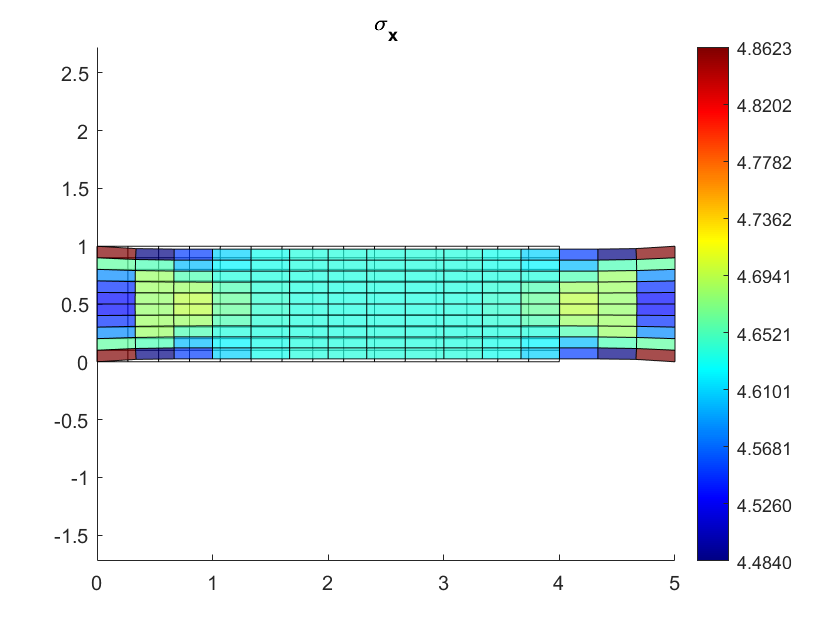
\includegraphics[width=1\textwidth]{Report/stretch.png}
        \caption{Loading conditions: horizontal stretch of the right edge}
        \label{fig:stretch}
    \end{subfigure}
    \hfill
    \begin{subfigure}[t]{0.49\textwidth}
        \centering
        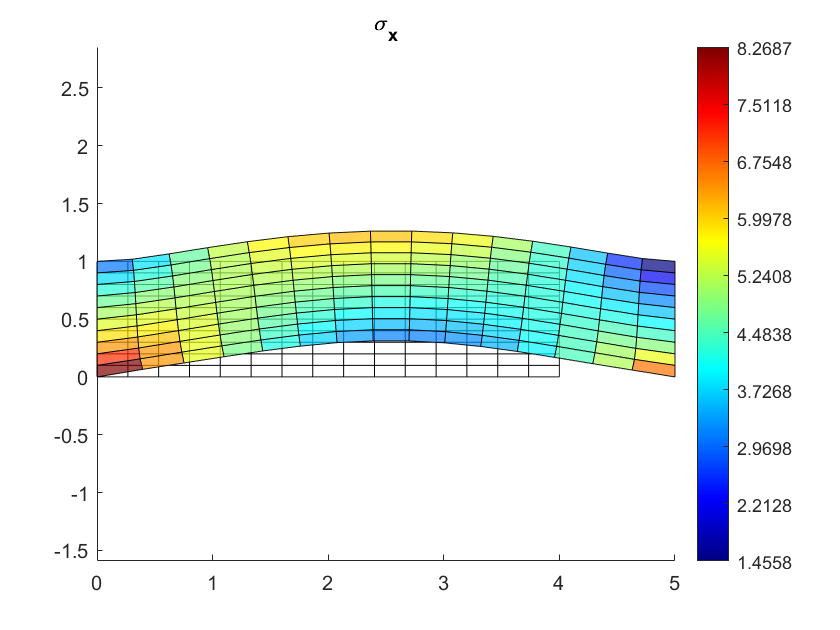
\includegraphics[width=1\textwidth]{Report/bending.png}
        \caption{Loading conditions: stretch + upwards distributed force on the top edge}
        \label{fig:bending}
    \end{subfigure}
    \caption{Plots of deformed bar}
    \label{fig:functionPlots}
\end{figure}
%
\end{document}